\documentclass{beamer}
\usepackage[utf8]{inputenc}

\usetheme{Madrid}
\usecolortheme{default}
\usepackage{amsmath,amssymb,amsfonts,amsthm}
\usepackage{txfonts}
\usepackage{tkz-euclide}
\usepackage{listings}
\usepackage{adjustbox}
\usepackage{array}
\usepackage{tabularx}
\usepackage{gvv}
\usepackage{lmodern}
\usepackage{circuitikz}
\usepackage{tikz}
\usepackage{graphicx}
\usepackage{amsmath}

\setbeamertemplate{page number in head/foot}[totalframenumber]

\usepackage{tcolorbox}
\tcbuselibrary{minted,breakable,xparse,skins}



\definecolor{bg}{gray}{0.95}
\DeclareTCBListing{mintedbox}{O{}m!O{}}{%
  breakable=true,
  listing engine=minted,
  listing only,
  minted language=#2,
  minted style=default,
  minted options={%
    linenos,
    gobble=0,
    breaklines=true,
    breakafter=,,
    fontsize=\small,
    numbersep=8pt,
    #1},
  boxsep=0pt,
  left skip=0pt,
  right skip=0pt,
  left=25pt,
  right=0pt,
  top=3pt,
  bottom=3pt,
  arc=5pt,
  leftrule=0pt,
  rightrule=0pt,
  bottomrule=2pt,
  toprule=2pt,
  colback=bg,
  colframe=orange!70,
  enhanced,
  overlay={%
    \begin{tcbclipinterior}
    \fill[orange!20!white] (frame.south west) rectangle ([xshift=20pt]frame.north west);
    \end{tcbclipinterior}},
  #3,
}
\lstset{
    language=C,
    basicstyle=\ttfamily\small,
    keywordstyle=\color{blue},
    stringstyle=\color{orange},
    commentstyle=\color{green!60!black},
    numbers=left,
    numberstyle=\tiny\color{gray},
    breaklines=true,
    showstringspaces=false,
}


\title 
{3.3.5}
\date{September 09,2025}


\author 
{Abhiram Reddy-AI25BTECH11021}



\begin{document}


\frame{\titlepage}
%------------------------------------
% Question frame
\begin{frame}{Problem statement}
Construct a $\triangle ABC$ in which 
\[
CA = 6\,cm, \quad AB = 5\,cm, \quad \text{and} \quad \angle BAC = 45^\circ.
\]
\end{frame}

% Step 1: Setup vectors
\begin{frame}{Step 1: Define Points and Vectors}
Place $A$ at origin: 
\[
\vec{A} = \begin{pmatrix}0 \\ 0\end{pmatrix}.
\]

Set $\vec{B}$ on x-axis since $AB=5\,cm$:
\[
\vec{B} = \begin{pmatrix}5 \\ 0\end{pmatrix}.
\]

Find $\vec{C}$ such that $|\vec{C}-\vec{A}|=6$ and $\angle BAC=45^\circ$.
\end{frame}

% Step 2: Calculate C using angle and length
\begin{frame}{Step 2: Calculate Coordinates of $C$}
Using trigonometry:
\[
\vec{C} = 6 \begin{pmatrix} \cos 45^\circ \\ \sin 45^\circ \end{pmatrix} 
= 6 \begin{pmatrix} \frac{\sqrt{2}}{2} \\ \frac{\sqrt{2}}{2} \end{pmatrix} 
= \begin{pmatrix} 3\sqrt{2} \\ 3\sqrt{2} \end{pmatrix}.
\]

Verify angle using dot product confirms $\angle BAC = 45^\circ$.
\end{frame}

% Step 3: Summary
\begin{frame}{Summary of Points}
\[
\boxed{
\vec{A} = \begin{pmatrix}0 \\ 0\end{pmatrix}, \quad
\vec{B} = \begin{pmatrix}5 \\ 0\end{pmatrix}, \quad
\vec{C} = \begin{pmatrix}3\sqrt{2} \\ 3\sqrt{2}\end{pmatrix}
}
\]

These points satisfy all given conditions.
\end{frame}

% C code part 1
\begin{frame}[fragile]{C Code: Dot Product and Magnitude}
\begin{lstlisting}[language=C]
#include <stdio.h>
#include <math.h>

double dotProduct(double A[], double B[]) {
    return A[0]*B[0] + A[1]*B[1];
}

double magnitude(double V[]) {
    return sqrt(V[0]*V[0] + V[1]*V[1]);
}
\end{lstlisting}
\end{frame}

% C code part 2
\begin{frame}[fragile]{C Code: Angle Calculation and Main}
\begin{lstlisting}[language=C]
double angleBetweenVectors(double A[], double B[]) {
    double dot = dotProduct(A, B);
    double magA = magnitude(A);
    double magB = magnitude(B);
    double cosTheta = dot / (magA * magB);
    if (cosTheta > 1.0) cosTheta = 1.0;
    else if (cosTheta < -1.0) cosTheta = -1.0;
    return acos(cosTheta) * (180.0 / M_PI);
}

int main() {
    double AB[2] = {5.0, 0.0};
    double AC[2] = {3.0 * sqrt(2), 3.0 * sqrt(2)};
    printf("Angle: %.2f degrees\n", angleBetweenVectors(AB, AC));
    return 0;
}
\end{lstlisting}
\end{frame}

% Python code part 1
\begin{frame}[fragile]{Python Code: Setup and Points}
\begin{lstlisting}[language=Python]
import matplotlib.pyplot as plt
import numpy as np

A = np.array([0, 0])
B = np.array([5, 0])
C = np.array([3 * np.sqrt(2), 3 * np.sqrt(2)])
\end{lstlisting}
\end{frame}

% Python code part 2
\begin{frame}[fragile]{Python Code: Plot Triangle}
\begin{lstlisting}[language=Python]
fig, ax = plt.subplots()

triangle_points = np.array([A, B, C, A])
ax.plot(triangle_points[:, 0], triangle_points[:, 1], 'b-', marker='o')

ax.text(A[0], A[1], 'A', fontsize=12, ha='right', va='top')
ax.text(B[0], B[1], 'B', fontsize=12, ha='left', va='top')
ax.text(C[0], C[1], 'C', fontsize=12, ha='left', va='bottom')
\end{lstlisting}
\end{frame}

% Python code part 3
\begin{frame}[fragile]{Python Code: Final Touches and Save}
\begin{lstlisting}[language=Python]
ax.set_aspect('equal', 'box')
ax.grid(True, linestyle='--', alpha=0.6)
ax.set_xlabel('x (cm)')
ax.set_ylabel('y (cm)')
ax.set_title('Triangle ABC with CA=6 cm, AB=5 cm, ∠BAC=45°')

padding = 1
min_x, max_x = min(A[0], B[0], C[0]) - padding, max(A[0], B[0], C[0]) + padding
min_y, max_y = min(A[1], B[1], C[1]) - padding, max(A[1], B[1], C[1]) + padding
ax.set_xlim(min_x, max_x)
ax.set_ylim(min_y, max_y)

plt.savefig('python_plot.png', dpi=300)
plt.show()
\end{lstlisting}
\end{frame}




\begin{frame}{Plot}
    \centering
    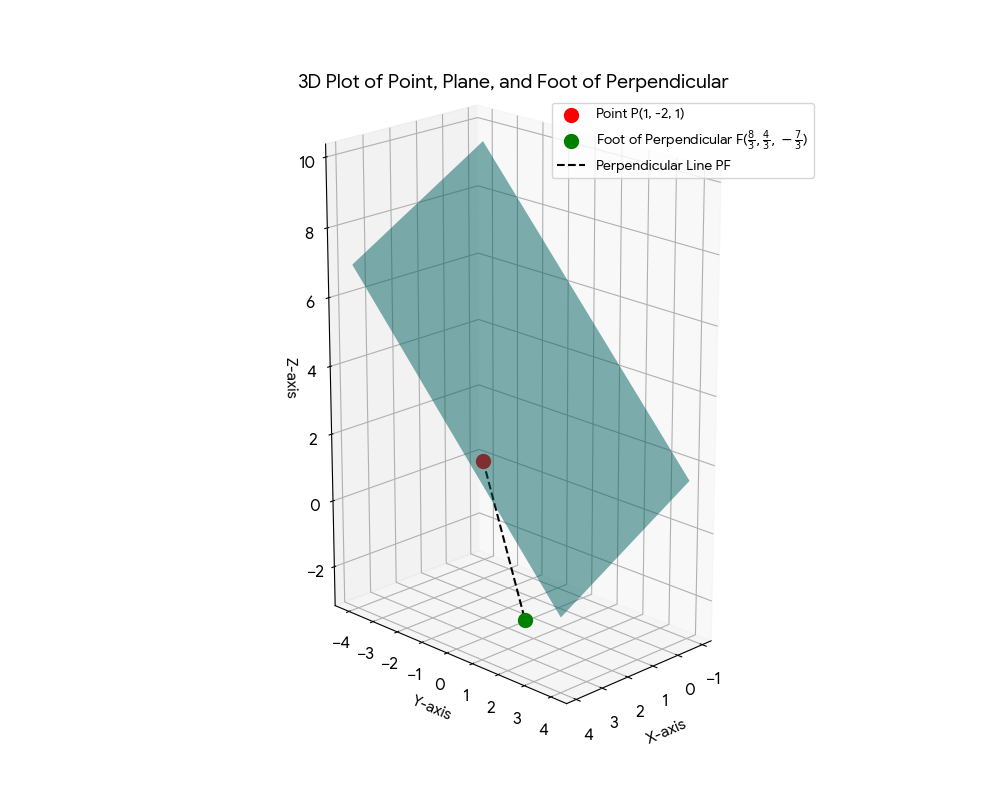
\includegraphics[width=\columnwidth, height=0.8\textheight, keepaspectratio]{figs/python_plot.png}     
\end{frame}


\end{document}